\section{Integración múltiple}
\stepcounter{sec}

En esta segunda parte del curso se estudiarán las nociones de campos conservativos. Para ello, necesitamos extender el concepto de integración a campos escalares y vectoriales.

En particular se introducirá la noción de integral de línea, integral de trayectoria, y finalmente la noción de integrales múltiples. Comenzaremos abordadno el estudio de la teoría de integración para campos escalares donde desarrollaremos la versión de la integración en el sentido de Riemann.

Finalmente cerraremos con tres teoremas centrales: El de Green, el de la divergencia y el de Stokes.

\subsection{Integrales de trayectoria}
\stepcounter{subsec}

Una integral de trayectoria es una integral cuyo dominio viene dado por una curva, la cual está definida por una función $\theta: [a,b] \rightarrow \R^n$. Esta curva va a venir dada por un vector de la siguiente manera:

\[
\theta(t) = (\theta_1(t), \dots, \theta_n(t))
\]

Pediremos también que $\theta \in C^2\left( [a,b] \right)$. Además, $\theta'(t) \neq 0$, $\forall~t \in [a,b]$.

De esta manera, la imagen $\theta(t) \subset \R^n$ la denotaremos por $C$, y esta será tal que no presenta ni picos ni se autointersecta. En este sentido, $C$ es una curva suave, simple y sin picos.

Bajo este contexto, podemos definir formalmente la integral de trayectoria:

\begin{defn}
    La \ul{integral de trayectoria} a lo largo de $C$ de la función $f: A \subset \R^n \rightarrow \R$ (con $A$ convexo y $C \subset A$) está denotada como
    
    \[
    \int_C fdS \quad \text{ó tambien} \quad \int_{\theta} fdS
    \]
    
    \noindent donde $dS$ es la variación sobre la curva.
    
    Y está definida como
    
    \[
    \int_{\theta} fdS = \int_a^b f\left( \theta(s) \right) \normaeuc{\theta'(s)}dS
    \]
    
    \noindent con $s \in [a,b]$.
\end{defn}

La motivación de esta definición viene de lo siguiente: Sea $N \in \N$, y $P_N \in P([a,b])$ una partición del intervalo $[a,b]$ tal que

\[
P_N = \{t_j\}_{j=1}^N, \quad \text{donde $a + \frac{j}{N}(b-a)$}
\]

\noindent con $j = 0, \dots, N$. Entonces por el \TVM~tendremos que

\[
\normaeuc{\theta(t_{j+1} + \theta(t_j))} = \left( \sum_{k=1}^n \left| \theta_k(t+1) - \theta_k(t_j) \right|^2 \right)^{1/2}
\]

\noindent donde cada $\theta_k(t_{j+1}) - \theta_k(t_j) = \theta'_k(\alpha_j)/N$ (con $\alpha_j \in (t_j, t_{j+1})$). De esta forma,

\begin{align*}
    S_N &= \sum_{j=0}^{N-1} \normaeuc{\theta(t_{j+1}) - \theta(t_j)} \\
        &= \sum_{j=0}^{N-1} \frac{\normaeuc{\theta'(\alpha_j)}}{N} 
\end{align*}

Ahora, al mirar el límite, la expresión anterior converge de la siguiente manera

\[
\limtoinfty{N}{S_N} = \int_a^b \normaeuc{\theta'(t)}dt \quad \footnotemark
\]\footnotetext{Donde la expresión $\int_a^b \normaeuc{\theta'(t)}dt$ es la longitud de arco de la curva $C$, cuando $n=1$.}

Un argumento análogo se realiza para la integral de trayectoria, pero esta vez estableciendo las sumas parciales:

\[
S_N(f, \theta) = \sum_{j=0}^{N-1} f \big( \theta(c_j) \big) \Delta S_j
\]

\noindent donde $\Delta S_j = \int_{t_j}^{t_{j+1}} \normaeuc{\theta'(u)} du$.

Al considerar el límite de estos factores, tendremos

\begin{align*}
    \limtoinfty{N}{S_N(f, \theta)} &= \limtoinfty{N}{\sum_{j=0}^{N-1} f \big( \theta(c_j) \big) \Delta S_j} \\
        &= \limtoinfty{N}{\sum_{j=0}^{N-1} \int_{t_j}^{t_{j+1}} f\big( \theta(c_j) \big) \normaeuc{\theta'(u)}du} \\
        &= \int_a^b f \big( \theta(u) \big) \normaeuc{\theta'(u)}du
\end{align*}

\noindent donde $c_j \in [t_j, t_{j+1}]$ para cada partición. Cuando efectivamente el límite anterior existe, entonces se le conoce como la integral de trayectoria de la función $f$ a lo largo de la curva que define $\theta$.

\subsection{Propiedades de las integrales de trayectoria}
\stepcounter{subsec}

Supongamos que $\lambda$ y $\theta$ son dos parametrizaciones que describen a una curva $C$ pero en sentidos contrarios. Entonces

\[
\int_{\theta} fdS = \int_{\lambda} fdS
\]

A continuación, solo consideraremos un caso especial de esta propiedad: Supongamos que tenemos dos valores $u, t \in [a,b]$ y la parametrización $\theta: [a,b] \rightarrow \R^n$, tendremos que

\[
\theta(u) = \left( x_1(u), \dots, x_n(u) \right)
\]

La idea será introducir una nueva función $u = u(t) = -t + b + a$, la cual no es otra cosa más que lo descrito en la figura \ref{fig:int-ab}.

\begin{figure}
    \centering
    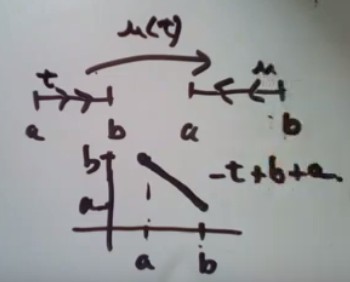
\includegraphics[scale=0.8]{img/int-ab.PNG}
    \caption{Vemos que se envía el punto $a$ al punto $b$ y viceversa. Si se recorre en intervalo $[a,b]$ en una dirección, pues pasa a ser recorrido en dirección contraria.}
    \label{fig:int-ab}
\end{figure}

Sea ahora $\lambda(t) = \theta\left( u(t) \right)$. Escribiendo explícitamente esta función tenemos

\[
\lambda(t) = \left( x_1(-t+b+a), \dots, x_n(-t+b+a) \right)
\]

\noindent y derivando,

\[
\lambda'(t) = -\left( x'_1(-t+b+a), \dots, x'_n(-t+b+a) \right) = -\theta'\left( u(t) \right)
\]

En conclusión $\lambda'(t) = -\theta'\left( u(t) \right)$ por lo tanto $\normaeuc{\lambda'(t)} = \normaeuc{\theta'(u)}$.

Así, nos queda que

\begin{align*}
    \int_{\lambda} fdS &= \int_a^b f\big( \lambda(t) \big)\normaeuc{\lambda'(t)} dt \\
        &= \int_a^b f\big(\theta(u)\big) \normaeuc{\theta'(u)}du \\
        &= \int_{\theta} fdS
\end{align*}

\noindent para $f: A \subset \R^n \rightarrow \R$ con $A$ convexo y que contiene a la curva $C$.

Ahora, otra propiedad que se puede verificar es la de linealidad:

\begin{teo}
    Sean $f,g$ acotadas tales que $f,g: A \subset \R^n \rightarrow \R$ con $A$ convexo. Sea $C \subset A$ una curva de clase $C^2([a,b])$. Supongamos que $c \in \R - \{0\}$. Bajo todas estas hipótesis, tenemos que

    \[
    \int_{\theta} \left( cf + g \right)dS = c\int_{\theta} fdS + \int_{\theta} gdS
    \]
    
    \noindent para todo $c \neq 0$\marginfootnote{La demostración de la linealidad queda como ejercicio. Para demostrarla, recordar que
    
    \[
    \int_{\theta} fdS = \limtoinfty{N}{\sum_{j=0}^{n-1}} \int_{t_j}^{t_{j+1}} f\left( \theta(c_j) \right) \normaeuc{\theta'(u)}du
    \]
    
    \noindent donde $c_j \in [t_j, t_{j+1}]$. La idea es utilizar las propiedades de linealidad de los límites y de la integral.}.
\end{teo}

Por último, estudiaremos un par de propiedades más:

\begin{teo}
    Sean $C \subset A \subset \R^n$ con $A$ convexo, y $f: A \rightarrow \R$ acotada. Sean $\lambda \in C^2([a,b])$ tal que $\lambda'(t) \neq 0$, $\forall~t \in (a,b)$ (inyectividad), esto garantiza la curva no presenta picos ni autointersecciones y $\mu: [a,b] \rightarrow C$ una reparametrización de $C$, es decir que $\exists~\phi:[\alpha,\beta] \rightarrow [a,b]$ sobreyectiva, continua, derivable tal que $\mu = \lambda \circ \phi$. Bajo todas estas condiciones, podemos concluir que

    \[
    \int_{\lambda} fdS = \int_{\mu} fdS
    \]
    
    Es decir, la integral de trayectoria no cambia con respecto a la parametrización presentada, siempre y cuando la reparametrización sea la apropiada. 
\end{teo}

\begin{proof}
    Para demostrar esto, utilizaremos el cambio de variable para integrales. En un principio, tenemos que por definición y aplicando el cambio de variable $u = \phi(t)$, $du = \phi'(t)dt$
    
    \begin{align*}
        \int_{\mu} fdS &= \int_{\alpha}^{\beta} f\big( \mu(t) \big)\normaeuc{\mu'(t)}dt \\
            &= \int_a^b f\big( \lambda(\phi(t)) \big)\normaeuc{\lambda'\big( \phi(t) \big) \cdot \phi'(t)}dt \\
            &= \int_a^b f\big( \lambda(u) \big)\normaeuc{\lambda'(u)}du \\
            &= \int_{\lambda} fdS
    \end{align*}
    
    De esta manera, $\int_{\mu} fdS = \int_{\lambda} fdS$.
\end{proof}

\begin{teo}
    Sea $\lambda \in C^2([a,b])$ una parametrización de una curva $C$ tal que $\lambda'(t) \neq 0$, $\forall~t \in [a,b]$ (con $\lambda$ recorriendo a $C$ una sola vez), sea $\mu$ otra parametrización de $C$ que la recorre $n$ veces. Entonces

    \[
    \int_{\mu} fdS = n \int_{\lambda} fdS
    \]
\end{teo}